\documentclass[border=4pt]{standalone}
\usepackage{tikz}
\usetikzlibrary{arrows.meta,positioning,shapes.multipart}
\begin{document}
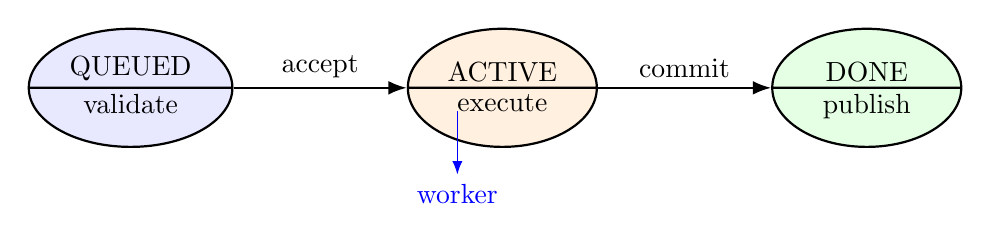
\begin{tikzpicture}[
  >=Latex,
  node distance=22mm,
  phase/.style={ellipse split,draw,thick,minimum width=24mm,
    minimum height=15mm,inner xsep=4pt,inner ysep=2pt,align=center}
]
  \node[phase,fill=blue!9] (queued) {QUEUED\nodepart{lower}validate};
  \node[phase,fill=orange!12,right=of queued] (active) {ACTIVE\nodepart{lower}execute};
  \node[phase,fill=green!10,right=of active] (done) {DONE\nodepart{lower}publish};

  \draw[-Latex,thick] (queued.east) -- node[above]{accept} (active.west);
  \draw[-Latex,thick] (active.east) -- node[above]{commit} (done.west);
  \draw[-Latex,blue] (active.lower) -- ++(0,-8mm) node[below]{worker};
\end{tikzpicture}
\end{document}
